\section{Hubbard model}\label{sec:hubbardModel}

The nearly free electron gas models the conduction bands of metals and alloys fairly accurately.
The high mobility of the electrons compared to the ions justifies two equivalent approximations, both giving essentially the same results \cite{ashcroft_solid_1976}.
The first idea is to treat the periodic potential created by the \emph{virtually} fixed ions (compared to the electrons) as a perturbation on the free electron gas.
Equivalently, we may imagine the system as a collection of tightly bond atoms, in which the electrons in the higher energy band hop from atom to atom.
Both these approaches lead to band theory, a framework which allows us to predict whether a material is a conductor or a insulator.
From the tight binding point of view, the effect of the electron mobility is the broadening of the atomic energy levels: the electrons in the solid occupy energy bands, rather than levels.
The partially filled band of highest energy is called the conduction band, since it is the band occupied by conduction electrons hopping from atom to atom.
However, in transition metal and rare-earths, as in some compounds containing these elements, apart from the conduction bands there are partially filled bands: $d-$ or $f-$bands.
The partial filling of these bands and the electron correlations within them are responsible for the characteristic properties of these solids.
Some of these properties are not explained by band theory, namely the Mott metal-insulator transition \cite{h_de_boer_semiconductors_1937, mott_discussion_1937, mott_basis_1949}.

\subsection{Electron correlations in narrow $d-$bands}

First, note that the effects of correlations cannot possibly be the same in narrow energy bands and in the free electron gas.
To see this, we may simply recall the shape of a $d-$wave function.

\begin{figure}[H]\label{fig:hydrogenWF}
\centering
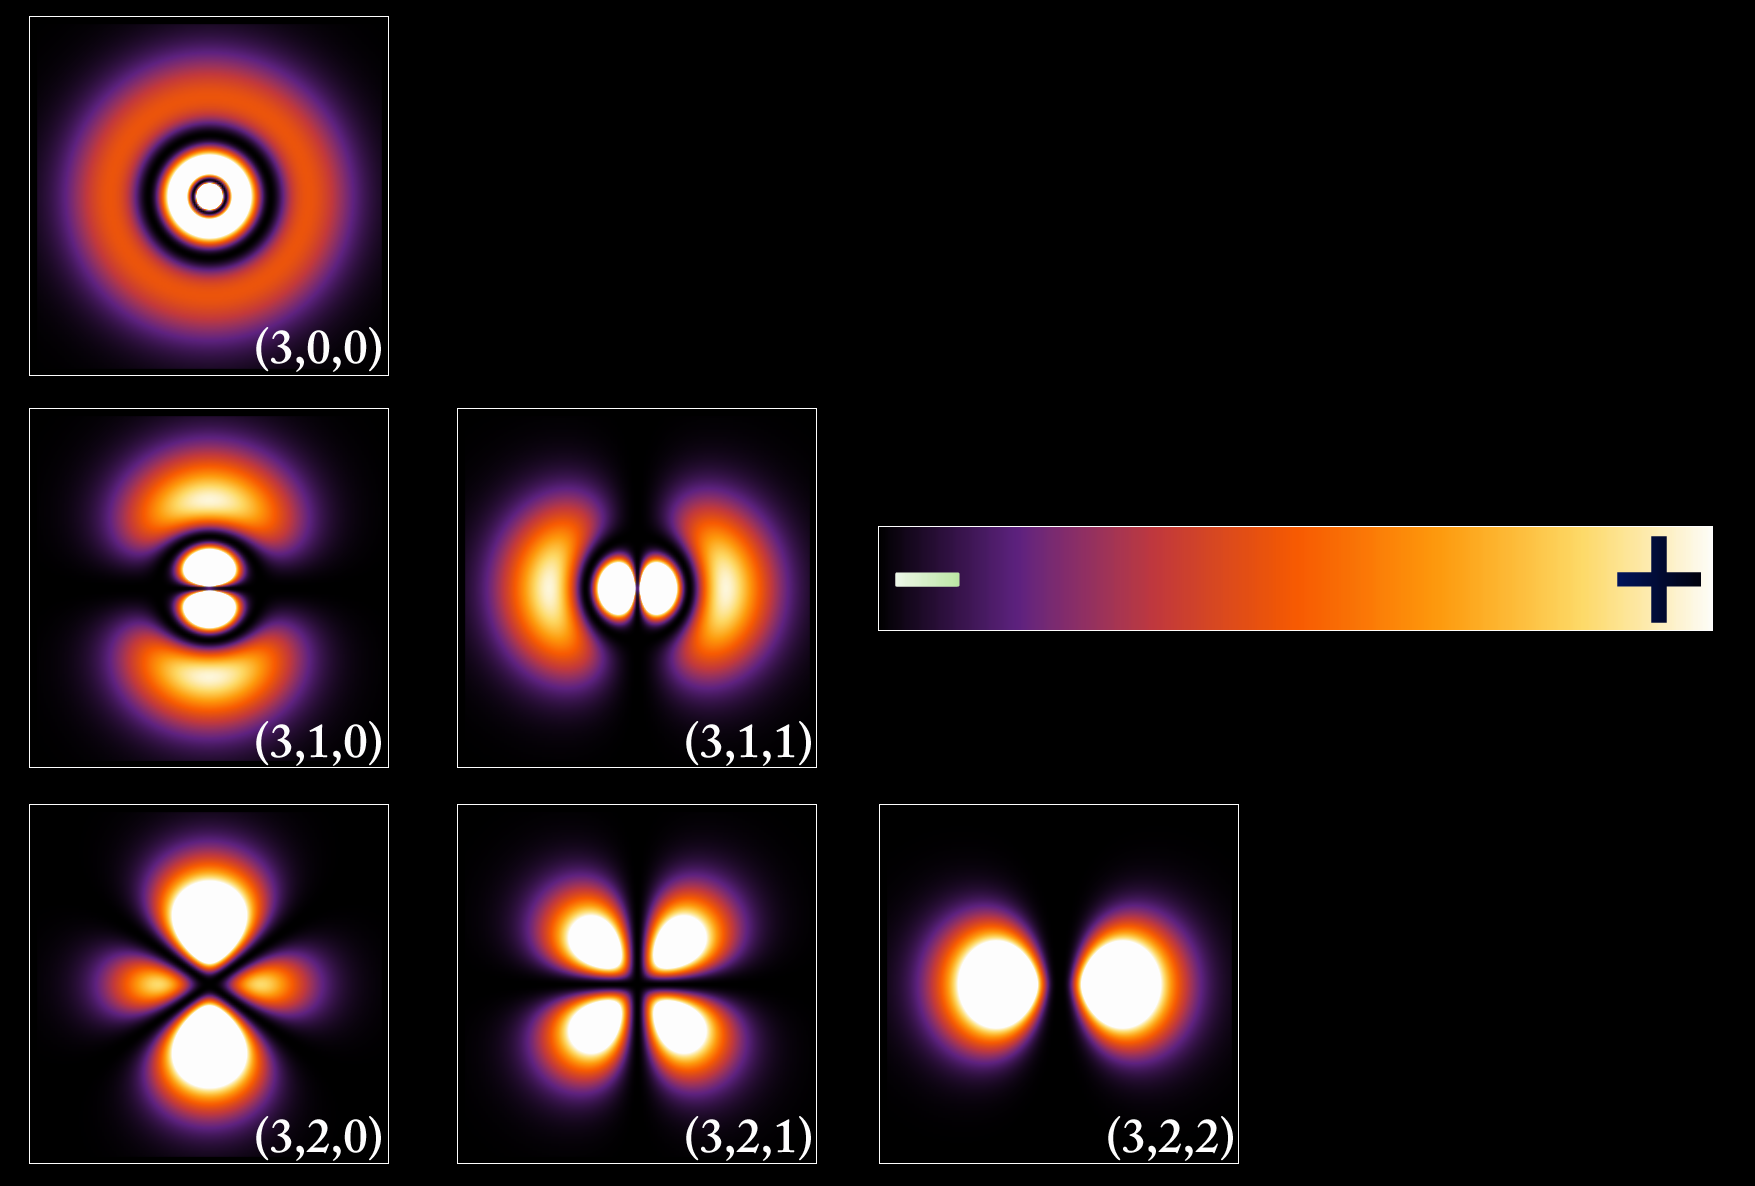
\includegraphics[width = 9cm]{Hubbard/Hydrogen_Density_Plots.png}
\caption[Hydrogen atomic wave functions.]{Probability density plots for different hydrogen orbital wave functions corresponding to quantum numbers $(n, l, m)$ for $n = 3$.
d-wave functions correspond to $l=2$. Note that the probability density is always higher in a region near the nucleus, and has a complicated shape, which will lead to a non-uniform distribution of electronic charge, as opposed to the case of the free electron gas. (adapted from \cite{hydrogen})}
\end{figure}

In a $d-$orbital, the electron charge density is concentrated near the nucleus.
In a solid, the electronic charge density should then also be concentrated near the nuclei, as long as the atomic description is useful, even if not completely correct\footnote{The electronic charge density is, of course, not actually defined in terms of a squared norm of the $d-$wave function for a narrow band. There is some broadening of the corresponding atomic energy level, and the wave function describing an electron is a Bloch wave function. Since the band is narrow, we assume that the atomic wave function description is still somewhat useful in a given range and we use it to provide a heuristic motivation for the non validity of the free electron assumption.}.
It is much smaller between atoms so that electrons do seem to belong to individual atoms in some sense.
For a $d-$band, we assume this description to hold to some extent since the band is narrow.
Thus, the fact that we may speak with some meaning of an electron belonging to a particular atom motivates a description from which the atomic characteristics of the solid emerge, in spite of the fact that the bandwidth of a $d-$band is still appreciable.
The point is that electrons in $d-$bands are certainly not well described by a free electron gas, which cannot possibly account for atomic-like behavior.

Experimentally, $d-$electrons of transition metals show hybrid behavior: sometimes they are accurately described by an ordinary band model, but there are occasions in which the atomic model is better.
For example, we see spin wave phenomena in ferromagnetic transition metals, and the susceptibilities of some of these metals depend strongly on temperature.
This is characteristic of an atomic (Heisenberg) model.
On the other hand, the $d-$electrons contribute significantly to the low temperature specific heat and sometimes the magnetic moments per atom of some transition metal ferromagnets are not integer multiples of the Bohr magneton.
This is characteristic of band theory\footnote{Think, for example, of a tight binding model. Electrons hop from atom to atom, and in general the spin of each atom depends on the particular electrons \say{belonging} to it at a given time. If we take an average of the total spin of each atom, we will in general not necessarily obtain an integer multiple of the Bohr magneton. If we simply had a collection of atoms, Hund's rule would apply, and each atom would have its spin aligned in a given direction. The average spin would then tend to be an integer multiple of the Bohr magneton.}.
Our theory of correlations should describe this balance between band-like and atomic-like behavior.

The atomic picture of a solid consists of an electron gas where ions are immersed.
The ions then interact in much the same way as they do in salts.
This extreme scenario is surely not even close to the true state of affairs since the number of $d-$electrons per atom is in general not an integer.
This motivates us to introduce a less restrictive model, which is not too far from the atomic model.
We shall assume that while $d-$electrons still have some band motion, they are strongly correlated with each other so that the solid retains some atomic-like behavior.
The correlations between electrons on different atoms are likely much weaker and we neglect them.

Let us now look at an example of the aforementioned circumstance.
Take a partially filled $d-$band of non-interacting electrons.
The spin of any given atom in the solid is just the total spin of all electrons on that atom.
It fluctuates both in magnitude and in direction, with a characteristic time that depends on how frequently $d-$electrons hop.
We can estimate the time interval between $d-$electron hopping events between atoms as a being of the order $\hbar / \Delta$, where $\Delta$ is the $d-$electron bandwidth.
The spin can thus be thought of as being associated to each individual (and constantly hopping) $d-$electron.

How do the electron interactions affect this picture?
We start by recalling Hund's rule: the nature of the  interactions between atoms leads to an alignment of the spins on each atom.
Since the atomic picture seems to prevail in our metal, we have reason to expect a similar effect to occur.
An atom with a total spin in some direction at a given time will tend to attract electrons with the spin on that direction and repel those with opposite spin.
This mechanism makes it unlikely for the spin of an atom to change much over time.
If the interactions between atoms are strong enough, the correlations become considerable and, making our statement  more precise, the total spin of an atom will persist for a time that is long compared with the $d-$electron hopping time.
Note that it is not the localization of the electrons that causes the spin state of the atom to persist.
The specific electrons belonging to a given atom change all the time as long as their spin is consistent with the total spin requirement imposed by Hund's rule.
For strong enough correlations, we may think of the spin as being associated to each atom, which opens up the possibility to describe the system using an atomic (Heisenberg) model, as we shall see later.

A theory of electron correlations in a narrow energy band should reduce to an atomic model in the appropriate limit, for example atoms that are so far apart on a lattice that they interact only very weakly.
Although we always keep in mind that we are focusing on $d-$electrons, we shall consider $s-$electrons in what follows for the sake of simplicity.
The important conclusions will not differ significantly.
We will use the "atomicity" of the electronic distribution to introduce an approximate representation of the electron interaction.
It turns out that this representation is mathematically much simpler to handle than the Coulomb interaction itself.

In short, our picture is the following: electrons hop rapidly from atom to atom in a band-like fashion, but their motion is correlated in such a way that atomic characteristics emerge.
The extent of atomic behavior depends, of course, on the strength of the interaction.

\subsection{Hubbard Hamiltonian}\label{subsec:hubbardHamiltonian}

Imagine a hypothetical partially filled narrow $s-$band with $n$ electrons per atom.
Suppose you have obtained Bloch wave functions $\psi_{\bm k}$ corresponding to energies $\varepsilon_{\bm k}$ by solving the Schr\"odinger equation for some spin-independent Hartree-Fock potential that accounts for the average interaction of the $s-$band electrons with electrons on other bands, and the interaction with the other $s-$electrons.
The electrons on the band evolve according to the Hamiltonian:

\begin{equation}\label{eq:startingHamiltonian}
\mathcal{H} = \sum_{\bm k \sigma} \bigg( \varepsilon_{\bm k} - \sum_{ \bm k'} \big( 2 V^{\bm k \bm k'}_{\bm k \bm k'} - V^{\bm k \bm k'}_{\bm k' \bm k} \big) \nu_{\bm k'} \bigg) c_{\bm k \sigma}^\dagger c_{\bm k \sigma} +  \frac{1}{2} \sum_{ \substack{\bm k_1 \bm k_2 \\ \bm k_1' \bm k_2'  \sigma_1 \sigma_2 } } V^{\bm k_1 \bm k_2}_{\bm k_1' \bm k_2'}
 c_{\bm k_1 \sigma_1}^\dagger c_{\bm k_2 \sigma_2}^\dagger c_{\bm k_2' \sigma_2} c_{\bm k_1' \sigma_1} ,
\end{equation}
where the $\bm k-$sums run over the first Brillouin zone.

The integrals are defined by

\begin{equation}\label{eq:integrals}
V^{\bm k_1 \bm k_2}_{\bm k_1' \bm k_2'} \equiv \left\langle \bm k_1 \bm k_2 \bigg| \frac{e^2}{r} \bigg| \bm k_1' \bm k_2' \right\rangle  =  e^2 \int \frac{\psi_{\bm k_1}^\star (\bm x) \psi_{\bm k_1'} (\bm x) \psi_{\bm k_2}^\star (\bm x') \psi_{\bm k_2'}(\bm x') }{| \bm x - \bm x' |} d\bm x d\bm x'
\end{equation}

The first term represents the band energies of the electrons minus their potential energy in the part of the Hartree-Fock field due to the electrons of the $s-$band itself.
The latter ensures that we do not overestimate the magnitude of the interactions between the electrons of the band: the Hartree-Fock field that specifies $\varepsilon_{\bm k}$ is computed taking into account these interactions, so if we didn't subtract it, we would count the energy of these interactions twice since they reappear in the last term, which  represents the interactions among all electrons in the system.
Furthermore, we assume that up and down spins are occupied equally, and $\nu_{\bm k}$ are the occupation numbers of the states of the band in the Hartree-Fock calculation. 

The term that we subtract in equation ($\ref{eq:startingHamiltonian}$) corresponds to the part of the interaction term which is already accounted for by the first diagonal \say{mean field} term.
Thus, it corresponds to the mean field expansion of the interaction term.
A generic way of writing the interaction term by gathering the $\bm k, \sigma$ indexes into a single index $\mu$ is

\begin{equation}\label{eq:vInt}
V_{\text{int}} = \frac{1}{2} V^{\nu\mu}_{\nu'\mu'} c_\nu^\dagger c_\mu^\dagger c_{\mu'} c_{\nu'} ,
\end{equation}
where the summation over repeated indexes is implied.
In appendix \ref{ap:hubbardObSol}, we obtain the mean field form of $V_{\text{int}}$ in the Hartree-Fock approximation.

Now consider the Wannier functions

\begin{equation}
\phi(\bm x) = N^{-1/2} \sum_{\bm k} \psi_{\bm k} (\bm x) , 
\end{equation}
where $N$ is the number of atoms.
We may write $\psi_{\bm k}$ as a combination of Wannier functions localized at each atom.

\begin{equation}
\psi_{\bm k} (\bm x) = N^{-1/2} \sum_i e^{i \bm k \cdot \bm R_i} \phi (\bm x - \bm R_i) ,
\end{equation}
where the sum runs over all atomic positions $\bm R_i$. 
Introducting the annihilation (creation) operators of an electron of spin $\sigma$ in the Wannier state $\phi (\bm x - \bm R_i)$ localized at site $i$, $c_{i\sigma}^{(\dagger)}$, we may write

\begin{equation}
c_{\bm k \sigma}^{(\dagger)} = N^{-1/2} \sum_i e^{i \bm k \cdot \bm R_i} c_{i\sigma}^{(\dagger)}
\end{equation}

Thus, the Hamiltonian becomes 

\begin{equation}
\mathcal{H} = \sum_{\substack{ i j \\ \sigma} } K_{ij} c_{i \sigma}^\dagger c_{j \sigma} + \sum_{\substack{i j k l \\ \sigma \sigma'} } \bigg[  \frac{1}{2} V^{i j}_{k l}
 c_{i \sigma}^\dagger c_{j \sigma'}^\dagger c_{l \sigma'} c_{ k \sigma} - \bigg( 2 V^{i j}_{k l} - V^{i j} _{l k} \bigg) \nu_{j l} c_{i \sigma}^\dagger c_{ k \sigma} \bigg]  ,
\end{equation}
where

\begin{equation}\label{eq:hopping_matrix}
K_{ij} = N^{-1} \sum_{\bm k} \varepsilon_{\bm k} e^{i \bm k \cdot ( \bm R_i - \bm R_j )}, \, \text{and} \, \, \nu_{j l} = N^{-1} \sum_{\bm k} e^{i \bm k \cdot ( \bm R_j - \bm R_l) }
\end{equation}

Now comes the crucial approximation.
For a narrow energy band, the Wannier functions $\phi$ nearly coincide with atomic $s-$functions.
For small bandwidth, these $s-$functions form an atomic shell whose radius is small compared with the spacing between atoms, that is, the lattice constant.
Thus, the integral $U = \left\langle i i \big| e^2 / r \big| i i \right\rangle$ should turn out to be much larger than all other integrals.
This suggests the seemingly crude approximation of neglecting all other integrals.
However, this approximation is not so radical as it could seem at first sight since the other integrals are indeed much smaller than $U$.
In fact, for example, for $3d$ electrons of transition metals they are smaller by about two orders of magnitude \cite{hubbard_electron_1963}.
Keeping only the terms in $U$ in the interaction part, we obtain

\begin{equation}
\mathcal{H} = \sum_{i, j, \sigma} K_{ij} c_{i\sigma}^\dagger c_{j\sigma} + \frac{U}{2} \sum_{i\sigma} n_{i\sigma} n_{i, -\sigma} - U \sum_{i, \sigma} \nu_{i, i} n_{i, \sigma}
\end{equation}
where $n_{i\sigma} = c_{i\sigma}^\dagger c_{i\sigma}$.
Note that $\nu_{i, i} = N^{-1} \sum_{\bm k} \nu_{\bm k} = n/2$, where $n$ is the electron density, which means that the last term is constant and may be dropped.
Now, the hopping matrix $\bm K$ can, in principle, be found by inverse Fourier transforming the dispersion relation $\varepsilon_{\bm k}$ of the equivalent interaction-free system, that we can assumed to be obtained experimentally or numerically.
In the purely tight binding view (with no $U$-term), we have a well defined crystal wavevectors that depends on the symmetry of the lattice, which may be written as Fourier transforms

\begin{equation}
\left| \bm k \right\rangle \equiv \frac{1}{N} \sum_{\bm r} e^{i\bm k \cdot \bm r} \left| \bm r \right\rangle
\end{equation}

Recalling the form of the hopping Hamiltonian (or the kinetic energy part in the Hubbard model)

\begin{equation}
\mathcal{H}_{K} = - \sum_{\bm r \bm r'} K (\bm r - \bm r') \left| \bm r' \right\rangle \left\langle \bm r \right|
\end{equation}
we can obtain the dispersion relation.

\begin{equation}
- \mathcal{H}_{K} \left| \bm k \right\rangle = \frac{1}{\sqrt{N}} \sum_{\bm r \bm r'} K ( \bm r - \bm r' ) e^{i \bm k \cdot \bm r} \left| \bm r' \right \rangle = \frac{1}{\sqrt{N}} \bigg( \sum_{\bm R} K(\bm R) e^{i\bm k \cdot \bm R} \bigg) \bigg( \sum_{\bm r'} e^{i\bm k \cdot \bm r'} \left| \bm r' \right\rangle \bigg) = \varepsilon_{\bm k} \left| \bm k \right\rangle
\end{equation}
and here we recognize the dispersion relation as the (negative) Fourier transform of the hopping

\begin{equation}
\varepsilon_{\bm k} = - \sum_{\bm R} K(\bm R) e^{i\bm k \cdot \bm R} 
\end{equation}

This gives us an interpretation of the $\bm K$ matrix: given the dispersion relation, and considering the solid to be well described by a tight binding model, we can easily obtain the matrix elements $K_{i j}$.

Let us now suppose that we have the simplest uniform nearest neighbor hopping model.
Going back to equation (\ref{eq:hopping_matrix}), and recalling that the sum on $\bm k$ is restricted to the first Brillouin zone, we obtain the usual tight binding result: $K_{\left\langle i j \right\rangle} = - t \in \mathbbm{R}$ and $0$ otherwise (i.e. $\bm K$ is a very sparse matrix that is only non-zero for $i, j$ nearest neighbors).
The Hubbard Hamiltonian is then

\begin{equation}\label{eq:hubbard_hamiltonian}
\mathcal{H} = - t \sum_{\left\langle i, j \right\rangle, \sigma} \bigg(c_{i,\sigma}^\dagger c_{j,\sigma} + c_{j,\sigma}^\dagger c_{i,\sigma} \bigg) + U \sum_{i} n_{i,\uparrow} n_{i\downarrow} -\mu \sum_i \bigg( n_{i,\uparrow} + n_{i,\downarrow} \bigg) ,
\end{equation}
where, for generality, we included an arbitrary chemical potential, so that we use the \ac{GCE}.

\subsection{Particle-hole symmetry}

In this section we examine a particularly relevant and unique symmetry of the Hubbard model.
The main idea is that, at half filling, the Hubbard Hamiltonian is invariant under a transformation which turns particles into holes and vice-versa.
\ac{PHS} allows us to relate the properties of the Hubbard Hamiltonian at different values of the parameters.
Moreover, it allows us to devise a mapping between the attractive ($U < 0$) and the repulsive ($U > 0$) models.
We will see later that this mapping is important in QMC simulations \cite{alavi_quantum_2016}.

We start our discussion with the concept of a bipartite lattice.
A lattice is said to be bipartite if it can be divided into two sublattices $\mathcal{A}$ and $\mathcal{B}$, such that the set of neighbors of a site in sublattice $\mathcal{A}$ belongs to sublattice $\mathcal{B}$.
For example, the square and honeycomb lattices are bipartite, whereas the triangular lattice is not.
In a bipartite lattice, \ac{AF} order is favored.
In contrast, AF order is frustrated on the triangular and other non bipartite lattices.

\begin{figure}[H]\label{fig:bipartite}
\centering
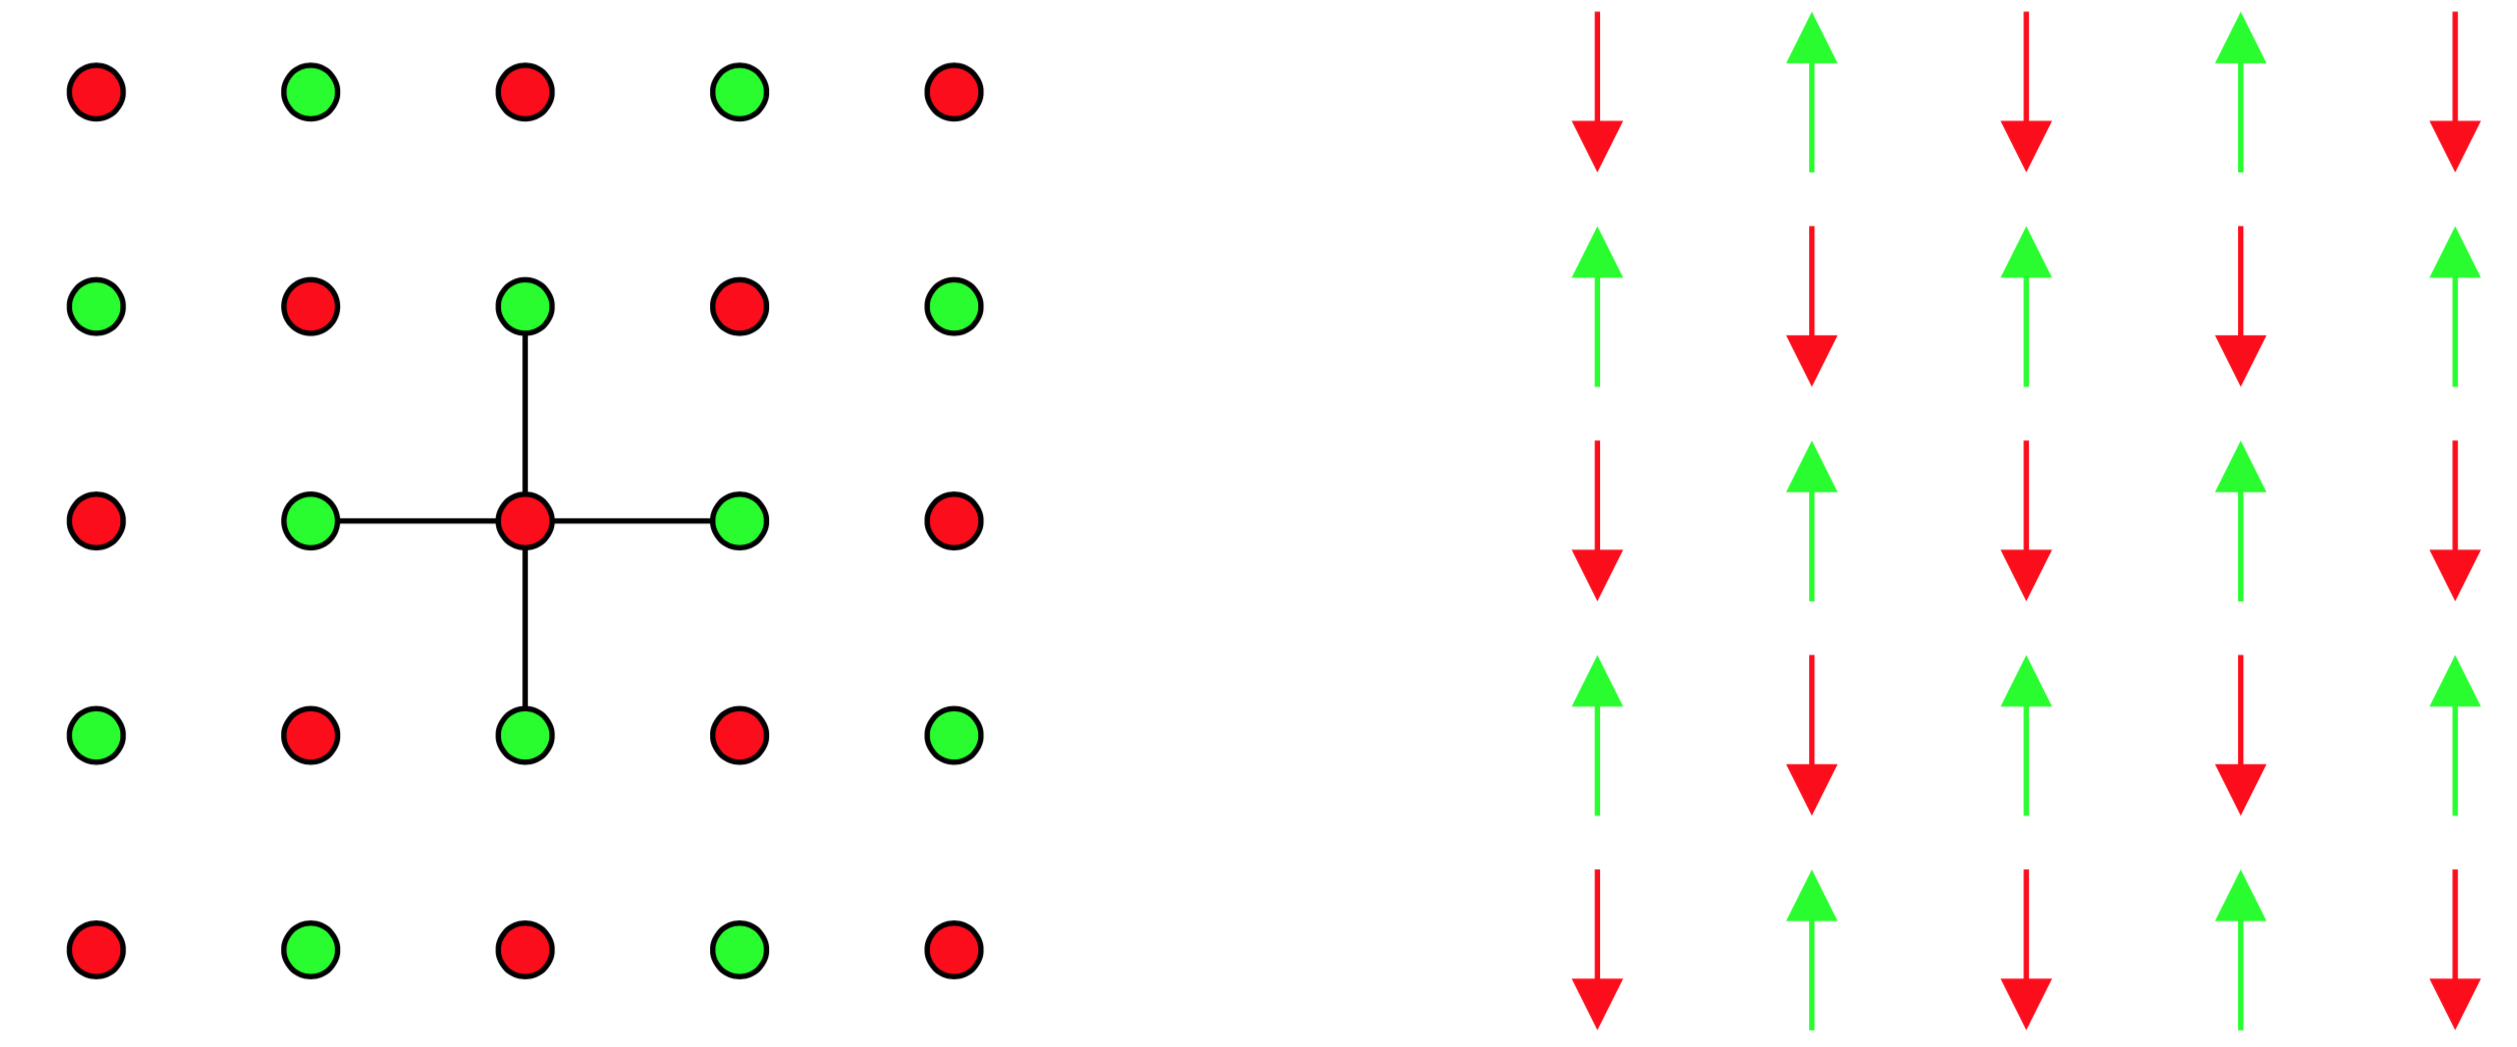
\includegraphics[width = 8cm]{Hubbard/bipartite}
\caption[Bipartite lattices and antiferromagnetic order.]{On the left, we see that the square lattice is bipartite.
The neighbors of a particular site in the red sublattice all belong to the green sublattice.
The picture on the right is meant to give some intuition on why the bipartite lattice favors \ac{AF} order.
We represent a configuration where fermions of a given spin have as their neighbors only fermions of opposite spin, which would be favored by Heisenberg exchange (taken from \cite{alavi_quantum_2016}). }
\end{figure}

Introducing a \ac{PHT},

\begin{equation}\label{eq:PHT}
d_{ i, \sigma}^\dagger = (-1)^i c_{i, \sigma} ,
\end{equation}
we exchange the role of annihilation and creation operators.
In fact, particles become holes and vice-versa: $d_{ i, \sigma}^\dagger d_{ i, \sigma} = 1 - c_{ i, \sigma}^\dagger c_{ i, \sigma} $, and the occupations $n = 0, 1$ are interchanged.
Consider a bipartite lattice.
Since in that case the factor $(-1)^i$ takes on $-1$ on one sublattice and $1$ on the other, the kinetic part of the Hamiltonian is invariant under a \ac{PHT}:

\begin{equation}
c_{i, \sigma}^\dagger c_{j, \sigma} + c_{j, \sigma}^\dagger c_{i, \sigma} \mapsto (-1)^{i+j} ( d_{i, \sigma} d_{j, \sigma}^\dagger + d_{j, \sigma} d_{i, \sigma}^\dagger ) = d_{j, \sigma}^\dagger d_{i, \sigma} + d_{i, \sigma}^\dagger d_{j, \sigma}
\end{equation}

The \ac{PHS} form of the kinetic term can be incorporated into the interaction term by a shift in the chemical potential and by adding a constant to the Hamiltonian.
First, note that the term

\begin{equation*}
U \bigg( n_{i,\uparrow} - \frac{1}{2} \bigg) \bigg( n_{i,\downarrow} - \frac{1}{2} \bigg)
\end{equation*}
is unchanged under a \ac{PHT}.
Expanding this term, we obtain $U n_{i,\uparrow} n_{i,\downarrow} - \frac{U}{2} (n_{i,\uparrow} + n_{i,\downarrow}) + \frac{U}{4}$, which indeed differs from the original interaction term by a shift in the chemical potential ($\mu \rightarrow \mu + U / 2$) plus a constant.
Thus, the particle-hole symmetric form of the Hamiltonian 

\begin{equation}
\mathcal{H} = -t \sum_{\left\langle i, j \right \rangle, \sigma} \bigg( c_{i,\sigma}^\dagger c_{j,\sigma} + c_{i,\sigma}^\dagger c_{j,\sigma} \bigg) + U \sum_{i} \bigg( n_{i,\uparrow} - \frac{1}{2} \bigg) \bigg( n_{i,\downarrow} - \frac{1}{2} \bigg) -\mu \sum_i \bigg( n_{i,\uparrow} + n_{i,\downarrow} \bigg)
\end{equation}
is completely equivalent to the original Hamiltonian.

Under a \ac{PHT}, the density, $\rho = \left\langle n_\uparrow + n_\downarrow \right\rangle$, transforms as $\rho \mapsto 2 - \rho$.
The Hamiltonian changes only in the chemical potential term: $\mu \mapsto -\mu$.
Thus, we have that $\rho (\mu) = 2 - \rho (-\mu)$, and at $\mu = 0$, we have half filling: $\rho = 1$.
This reasoning is valid for any $\beta$, $t$, or $U$, which implies that the phase diagram of the Hubbard model must be symmetric about half filling.
Suppose you added next nearest neighbor (NNN) hoppings $t'$\footnote{On the square lattice, this corresponds to connecting sites across the diagonal of each square.}.
Then, \ac{PHS} would be broken, and the phase diagram would no longer be symmetric about $\mu = 0$.
Indeed, a modified version of the Hubbard model with NNN hoppings is often used to model cuprate superconductors, and this lack of symmetry is consistent with the fact that hole- and electron-doped cuprates have different properties. 
\ac{PHS} is also broken for the triangular lattice with non uniform hoppings we shall consider later when modelling \acp{TMD}.